\chapter{پیش‌درآمد}
\pagebreak
\section{مقدمه}
در فصل پیش رو، مقدمه‌ای بر مسئله‌ی درک زبان طبیعی بیان می‌شود. در ادامه، از کاربرد آن در سیستم‌های گوناگون و سیستم‌های امروزی سخن گفته شده و اهمیت آن تبیین گردیده است. در این راستا،  ابتدا تعریف مسئله‌ی درک زبان طبیعی و دو وظیفه‌ای که پایه‌های مسئله را تشکیل داده‌اند گفته شده است و در ادامه، اهمیت مسئله و کاربرد آن را در دنیای واقعی تشریح شده است.
\section{تعریف مسئله: طراحی یک مدل برای درک زبان طبیعی}
سیستم گفت‌وگو\LTRfootnote{Dialogue System}
 یک برنامه‌ی رایانه‌ای است که برای تعامل با انسان از طریق متن یا صوت طراحی شده است. سیستم گفت‌وگو از طریق شبیه‌سازی مکالمه با انسان، امکان خودکارسازی امور را افزایش می‌دهد. در نتیجه، استفاده از آن باعث سادگی تعامل انسان با رایانه و افزایش دسترسی به اطلاعات و امکانات سیستم رایانه‌ای می‌شود.
در یک سیستم گفت‌وگو، کاربر سؤالی را به زبان طبیعی مطرح می‌کند که پاسخ آن درون پایگاه دانش قرار دارد. وظیفه‌ی سیستم گفت‌وگو این است که هدف و اطلاعات مهم معنایی را از سؤال استخراج کرده و ضمن پیدا کردن پاسخ مناسب از پایگاه دانش، جوابی فراخور را به کاربر نمایش دهد. بدین منظور، مطابق شکل \ref{Fig:dialoguesystem}، در ابتدا سوال کاربر وارد واحد درک زبان طبیعی\LTRfootnote{Natural Language Understanding} می‌شود. این واحد هدف و ترکیبات معنایی موجود در سوال را استخراج کرده و در اختیار واحد مدیریت مکالمه\LTRfootnote{Dialogue Management Unit} قرار می‌دهد. واحد مدیریت مکالمه، وظیفه‌ی نگهداری و ردیابی مکالمه‌ی کاربر و همچنین تعامل با پایگاه دانش را برعهده دارد.  این واحد با توجه به سیاست‌‌های\LTRfootnote{Policy} موجود، تصمیمی را اتخاذ کرده و آن را در اختیار واحد تولید زبان\LTRfootnote{Language Generation Unit} قرار می‌دهد، تا این واحد اقدام به تولید پاسخ کند. توانایی کاربر به سؤال کردن محدود نمی‌شود؛ بلکه می‌تواند درخواست انجام عمل نیز بدهد. در این صورت، به جای تولید پاسخ به زبان طبیعی، عمل مناسب توسط سیاست‌های موجود در پایگاه دانش مشخص شده و به واحد مدیریت مکالمه ابلاغ می‌شود.
\begin{figure}[!htb]
	\centering
	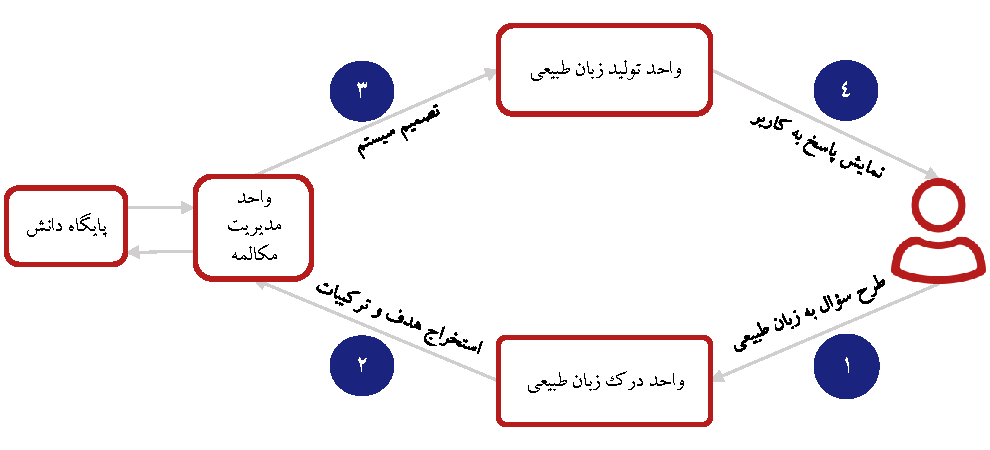
\includegraphics[scale=0.9]{Figures/dialoguesystem.pdf}
	\caption{فرایند عملکرد سیستم‌های گفت‌وگو}
	\label{Fig:dialoguesystem}
\end{figure} 


همانطور که در شکل \ref{Fig:dialoguesystem} مشهود است، درک زبان طبیعی نخستین بخش در چرخه‌ی عملکرد سیستم گفت‌وگو است. این امر بیانگر نقش حیاتی این سیستم است؛ به نحوی که نقص در عملکرد این بخش منجر به ایجاد گلوگاه\LTRfootnote{Bottleneck} برای سایر اجزاء سیستم می‌شود.
 درک زبان طبیعی شامل دو وظیفه‌ی "تشخیص هدف"\LTRfootnote{Intent-Detection} و "پرکردن جای خالی"\LTRfootnote{Slot-Filling} است.  غایت در وظیفه‌ی تشخیص هدف، پیش‌بینی منظور کاربر از سوال مطرح شده است. همچنین، پرکردن جای خالی به معنای استخراج اطلاعات معنایی\LTRfootnote{Semantic Information} از درون جمله است. اطلاعات معنایی، واژه‌هایی از جمله هستند که دارای نام، کد، زمان و اطلاعاتی بوده که به تکمیل وظیفه کمک می‌کنند. پر کردن جای خالی را می‌توان به عنوان یک مسئله‌ی برچسب‌زنی توالی\LTRfootnote{Sequence Labeling}، و تشخیص هدف را به عنوان یک مسئله‌ی کلاس‌بندی\LTRfootnote{Classification} تعریف کرد.
 
 
برای تعریف رسمی مسئله، تعداد واژه‌ها در زبان کاربر با $V$، تعداد برچسب‌های یکتا با $T$، تعداد اهداف یکتا در مجموعه داده با $I$ و تعداد واژه‌های سؤال با $n$، نمایش داده می‌شود. در این صورت، کاربر سوال خود را در قالب $Q=\{q_{1},q_{2},q_{3},\cdots,q_{n}\} , q_{i}\in\mathbb{W}^{V}$ مطرح می‌کند. واحد درک زبان طبیعی به ازاء هر $Q$، یک هدف $i\in\mathbb{W}^{I}$، و ترتیب $S$ که به صورت $S=\{s_{1},s_{2},s_{3},\cdots,s_{n}\} , s_{i}\in\mathbb{W}^{T}$ تعریف می‌شود را، تولید خواهد کرد. جدول \ref{Tab:atis} نمونه‌ای از سوال کاربر، برچسب مورد انتظار و هدف مورد نظر را از مجموعه داده‌ی \lr{ATIS} نمایش می‌دهد. در این مثال، برچسب‌های $O$ به معنای عدم وجود ترکیبات مهم معنایی در واژه است. ترکیباتی که حاوی اطلاعات مهم باشند، با برچسبی متناسب با معنای آن واژه، برچسب‌زنی می‌شوند. این برچسب‌ها از نظر معنایی هم‌راستا با هدف کاربر هستند. 


\begin{table*}[ht]
	\begin{latin}
		\input{Tables/atis_example.txt}
	\end{latin}
	
	\caption{
		نمونه‌ی سؤال کاربر، برچسب‌های صحیح و هدف مورد نظر کاربر از مجموعه داده‌ی \lr{ATIS}.
	}
	\label{Tab:atis}
\end{table*}
به منظور انجام دو وظیفه‌ی یاد شده، لازم است که مدل بر روی مجموعه داده‌ی مشخصی آموزش داده شود. 
هدف اصلی این پایان‌نامه، طراحی مدلی است که بتواند حل مسئله‌ی مذکور را یاد بگیرد؛ یعنی در مواجه با سؤال دیده نشده، هدف صحیح و اطلاعات معنایی موجود در جمله را استخراج کرده و در اختیار سایر بخش‌های سیستم گفت‌وگو قرار دهد.
طراحی یک مدل درک زبان طبیعی که در شرایط مختلف خوب عمل کند، یک چالش کلیدی است؛ چراکه زبان طبیعی پیچیده و غیرقابل پیش‌بینی است. این ویژگی زبان طبیعی باعث شده است که رایانه برای درک جمله و هدف کاربر با دشواری روبرو شود. همچنین مدل درک زبان باید همواره به‌روزرسانی و بازآموزی شود تا با تغییرات زبان و درخواست‌های جدید کاربران سازگار بماند. برای ساخت یک مدل درک زبان طبیعی، باید حجم زیادی داده جمع‌آوری و علامت‌گذاری شود. این علامت‌گذاری‌ها شامل هدف کاربر از نوشتن جمله و موجودیت‌های درون جمله می‌شوند.

\section{اهمیت مسئله}
با رشد سریع تلفن‌های هوشمند، استفاده از ابزارهای مبتنی بر سیستم گفت‌وگو نیز به طرز چشم‌گیری افزایش داشته است. استفاده از سیستم گفت‌وگو می‌تواند با کاهش ترافیک خطوط ارتباطی شرکت‌ها، هزینه‌ی عملیاتی\LTRfootnote{Operational Cost} آن‌ها کاهش دهد. از طرف دیگر سرعت پاسخگویی یک سیستم گفت‌وگو، باعث راحتی کار کاربر برای دریافت خدمت و افزایش رضایتمندی او می‌شود. در ادامه به معرفی برخی از ابزارهای دیجیتال که از سیستم گفت‌وگو بهره برده‌اند پرداخته می‌شود.
\\
	\textbf{\ding{118} خدمات مشتری به صورت خودکار:}
می‌توان از یک سیستم گفت‌وگو برای ارائه خدمات به صورت خودکار به مشتریان در وب‌سایت‌ها استفاده کرد. چنین سیستمی قادر است به سوالات متداول پاسخ‌های خودکار ارائه دهد، مشتریان را به بخش مربوطه هدایت کند و اطلاعاتی سودمند برای کسانی که کمک بیشتری می‌خواهند ارائه دهد.
\begin{figure}[!htb]
	\centering
	\subfloat[دستیار دیجیتال مسترکارت]{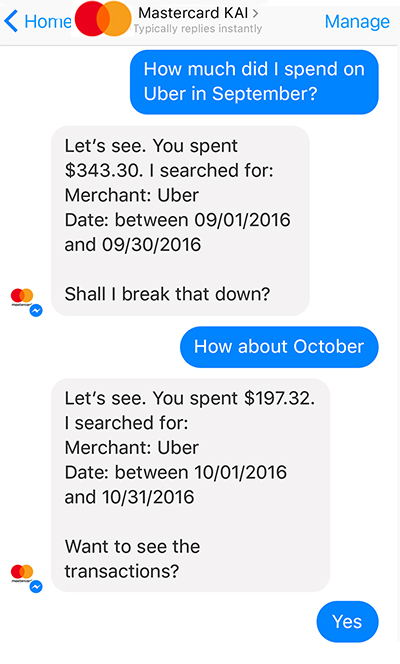
\includegraphics[scale=0.45]{Figures/mastercard.jpg}}
	\quad
	\subfloat[دستیار شخصی گوگل]{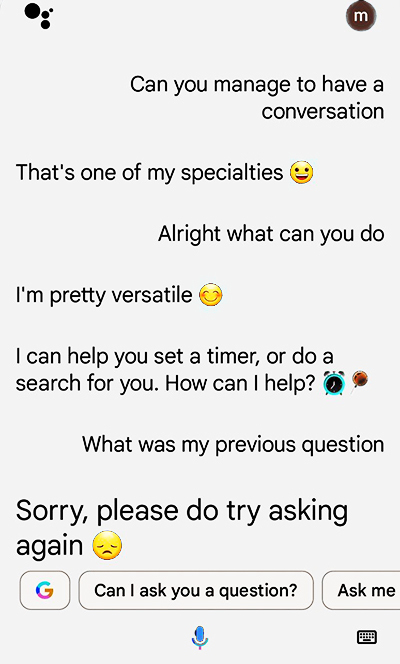
\includegraphics[scale=0.45]{Figures/assistant.jpg}}
	\caption{
		دستیار دیجیتال استفاده شده در وبسایت‌ها برای بهبود تجربه‌ی کاربری مشتریان
	}
	\label{Fig:DialoguesystemExamples۲}
\end{figure}
\\
\textbf {\ding{118} دستیار شخصی دیجیتال:}
دستیارهای شخصی دیجیتال، توانایی انجام کارهای روزمره مانند پخش موسیقی، تنظیم یادآور و کنترل ابزارهای هوشمند را دارند. بهره‌وری از این امکانات، منجر به افزایش کیفیت زندگی کاربران می‌شود. از نمونه‌های امروزی این دستیارها می‌توان به دستیار گوگل در شکل \ref{Fig:DialoguesystemExamples۲}، الکسا و سیری اشاره کرد.
\\
\textbf {\ding{118} دستیار شخصی خرید:}
این نوع از دستیارها در وبسایت‌های فروشگاهی به منظور فراهم کردن تجربه‌ی خرید بهتر برای کاربران مورد بهره‌وری قرار می‌گیرند. کاربر می‌تواند به جای ساعت‌ها گشتن در وبسایت برای یافتن محصول، با ارائه‌ی درخواست خود به دستیار خرید، سریع‌تر به محصول مورد نظرش برسد. چنین سیستمی قادر به ارائه پیشنهادهای ویژه به کاربر به منظور افزایش احتمال خرید او نیز هست. شکل \ref{Fig:DialoguesystemExamples} چنین سیستمی را در فروشگاه مایکروسافت و شرکت راه‌آهن امترک نمایش می‌دهد.
\\
\textbf {\ding{118} تدریس خصوصی برخط:}
این ابزار شامل یک سیستم گفت‌وگو برای تفسیر سوالات دانش‌آموزان و ارائه پاسخ‌های مناسب می‌باشد. قادر به ارائه راهنمایی و پشتیبانی شخصی به دانش آموزان است و می‌تواند به آن‌ها به منظور تسلط بر مطالعات خود کمک کند.
\begin{figure}[!htb]
	\centering
	\subfloat[دستیار دیجیتال فروشگاه مایکروسافت]{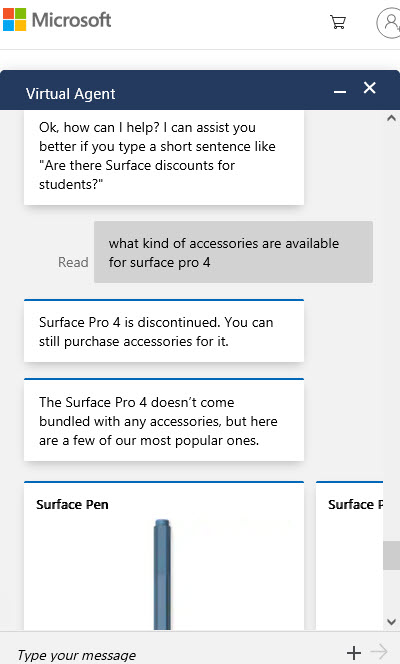
\includegraphics[scale=0.6]{Figures/microsoft.jpg}}
	\quad
	\subfloat[پشتیبان دیجیتال شرکت راه‌آهن امترک]{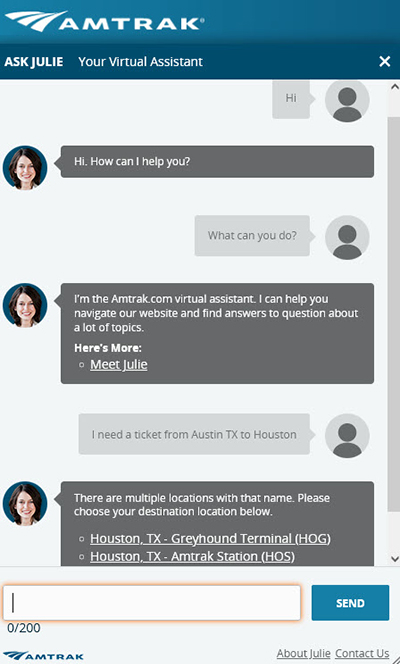
\includegraphics[scale=0.6]{Figures/amtrak.jpg}}
	\caption{
		دستیار دیجیتال استفاده شده در وبسایت‌ها برای بهبود تجربه‌ی کاربری مشتریان
	}
	\label{Fig:DialoguesystemExamples}
\end{figure}
\\
\textbf{\ding{118} تعامل در رسانه‌های اجتماعی:}
برای ارائه خدمات تعامل در شبکه‌های اجتماعی می‌توان از یک سیستم گفت‌وگو استفاده کرد. این سیستم قادر است سوالات مشتریان را در کانال‌های شبکه‌های اجتماعی تفسیر کرده و به شیوه‌ای مناسب به آن‌ها پاسخ دهد. همچنین، این سیستم می‌تواند واژه‌های کلیدی و عباراتی را که نشان‌دهنده احساسات مثبت یا منفی هستند، شناسایی کرده و به آن پاسخ دهد. از موارد پیاده‌سازی شده می‌توان به ربات شرکت تلوزیونی ام‌تی‌وی، و سامسونگ استرالیا نام برد \cite{socialchatbot}.

از طرف دیگر، مدلی که توانایی حل دو مسئله‌ی تشخیص هدف کاربر و استخراج روابط معنایی را بر داشته باشد، در بسیاری از وظایف دیگر پردازش زبان طبیعی نیز کاربرد دارد. همانطور که گفته شد، تشخیص هدف کاربر یک مسئله‌ی کلاس‌بندی است. از سایر وظایف کلاس‌بندی در زبان طبیعی که می‌توانند از معماری ارائه شده بهره ببرند، می‌توان به تحلیل احساسات\LTRfootnote{Sentiment Analysis}، تشخیص کلام نفرت‌افکن\LTRfootnote{Hate-Speech}، تشخیص اخبار جعلی\LTRfootnote{Fake-News Detection} و تشخیص موضع\LTRfootnote{Stance Detection} اشاره کرد. از سوی دیگر، مسئله‌ی پرکردن جای خالی یک مسئله‌ی برچسب‌زنی توالی است. سایر زمینه‌هایی که می‌توانند معماری مشترکی با این وظیفه داشته باشند شامل استخراج موجودیت، ابهام زدایی معنای واژه و برچسب زنی اجزاء سخن هستند. تشابه ساختار ورودی-خروجی و انتظارات مشابهی که از مدل زمینه‌های ذکرشده وجود دارد، باعث برجسته شدن فواید یک مدل قدرتمند در زمینه‌ی درک زبان طبیعی می‌شود.
\section{اهداف پژوهش}
به منظور آشنایی با محتوای پژوهش، باید با اهداف مورد نظر آن آشنا شد. در ادامه، اهدافی که این پایان‌نامه حول آن شکل گرفت معرفی می‌شوند.\\
\textbf{اول) }بسیاری از مدل‌های ارائه شده برای درک زبان طبیعی، همچنان از شبکه‌ی \lr{LSTM} به عنوان رمزنگار یا رمزگشا در مدل خود استفاده می‌کنند. نخستین هدف این پژوهش، ارائه‌ی مدلی است که شبکه‌های عصبی بازگشتی را کاملا کنار گذاشته و با ترنسفورمرها جابجا کند.\\
\textbf{دوم) }استفاده از ترنسفورمر، ضعف‌های ذاتی شبکه‌ی عصبی بازگشتی را پوشش می‌دهد. با این وجود شاید به نظر برسد که استفاده از شبکه‌ی عصبی کانولوشنی دیگر در رمزنگار ضروری نیست. هدف دوم پژوهش، بررسی عملکرد ترکیب شبکه‌ی عصبی بازگشتی، با ترنسفورمر در رمزنگار است.\\
\textbf{سوم) }تراز بودن مدل، موضوعی مهم در وظیفه‌ی برچسب زنی توالی است؛ اما تاکنون شیوه‌ای برای تراز کردن رمزگشای ترنسفورمر ارائه نشده است. هدف دوم پژوهش، ارائه کردن مدلی برای تراز کردن رمزگشای ترنسفورمر است.\\
\textbf{چهارم) }مدل زبانی بِرت انقلابی در یادگیری انتقالی در زبان طبیعی ایجاد کرد. پیش از برت، مدل زبانی اِلمو ارائه شده بود اما به اندازه‌ی برت مورد بررسی قرار نگرفت. علاوه بر این، تعداد کارهای اندکی در درک زبان طبیعی از المو استفاده کردند. در این کار قصد داریم عملکرد مدل زبانی المو را در شرایط یکسان، بر روی وظیفه‌ی درک زبان طبیعی بسنجیم. \\
\textbf{پنجم)} برخی از کارهای پیشین، مدل زبانی را به عنوان رمزنگار، و برخی دیگر به عنوان تعبیه‌ی کلمات استفاده کردند. یکی دیگر از اهداف این پژوهش، مقایسه‌ی این دو شیوه برای به کار گیری مدل زبانی است.\\
\textbf{ششم)} آخرین هدف در این پایان‌نامه، معرفی یک مدل جدید است که بر روی مجموعه داده‌ی \lr{SNIPS}‌ و یا \lr{ATIS}، بیشترین دقت را داشته باشد.
\section{ساختار پایان‌نامه}
در ادامه‌ی این پایان نامه، ابتدا در فصل ۲، به مفاهیم پایه‌ی درک زبان طبیعی و شبکه‌ی عصبی پرداخته می‌شود. در ادامه‌ی فصل ۲، مطالبی برای آشنایی با شبکه‌های عصبی ارائه می‌شود. سپس انواع شبکه‌های عصبی که در زمینه‌ی درک زبان طبیعی و وظایف مرتبط، از آن‌ها استفاده شده، معرفی می‌شوند. علت توصیف گسترده‌ی این شبکه‌ها، ماهیت کار این پایان‌نامه است؛ چراکه در این پایان‌نامه، یکی از کارهایی که صورت گرفته، تلاش برای پوشش ضعف شبکه‌های مورد استفاده است. در فصل ۳، یک دسته‌بندی کلی از کارهای پیشین در نظر گرفته شده، و در قالب این دسته‌بندی، پیشین مورد بررسی قرار گرفته‌اند. در فصل ۴،  مدل پیشنهادی این پایان‌نامه، یعنی \lr{CTran}، و اجزای سازنده‌ی آن معرفی شده‌اند. در فصل ۵، به تنظیمات به کار برده شده برای آموزش مدل، مجموعه داده‌های مورد استفاده، نتایج مدل پیشنهادی روی مجموعه داده‌ها و تجزیه و تحلیل نتایج پرداخته می‌شود. در فصل ۶، یک نتیجه‌گیری از آزمایش‌های صورت گرفته ارائه می‌شود. در پایان، کارهایی که می‌توان در آینده برای بهبود مدل پیشنهادی انجام داد، ذکر می‌شوند.


